% Source: Code/xband-radar-sim/docs/radar_simulation_technical.tex
% Description: 2D radar Point Spread Function. The PSF is narrower in range (from pulse compression) and wider in azimuth (from beamwidth).

\documentclass[border=4pt]{standalone}
\usepackage{algpseudocode}
\usepackage{amsmath,amssymb,amsfonts}
\usepackage[T1]{fontenc}
\usepackage{graphicx}
\usepackage{pgfplots}
\usepackage{tikz}
\usepackage{xcolor}
\pgfplotsset{compat=1.18}
\usetikzlibrary{arrows.meta,positioning,shapes.geometric,calc,patterns,decorations.pathmorphing,3d,angles,quotes}

\definecolor{radargreen}{RGB}{0,255,0}
\definecolor{raycolor}{RGB}{255,165,0}
\definecolor{targetcolor}{RGB}{255,0,0}
\definecolor{groundcolor}{RGB}{139,90,43}
\definecolor{skycolor}{RGB}{135,206,235}
\definecolor{beamcolor}{RGB}{255,255,0}


\begin{document}
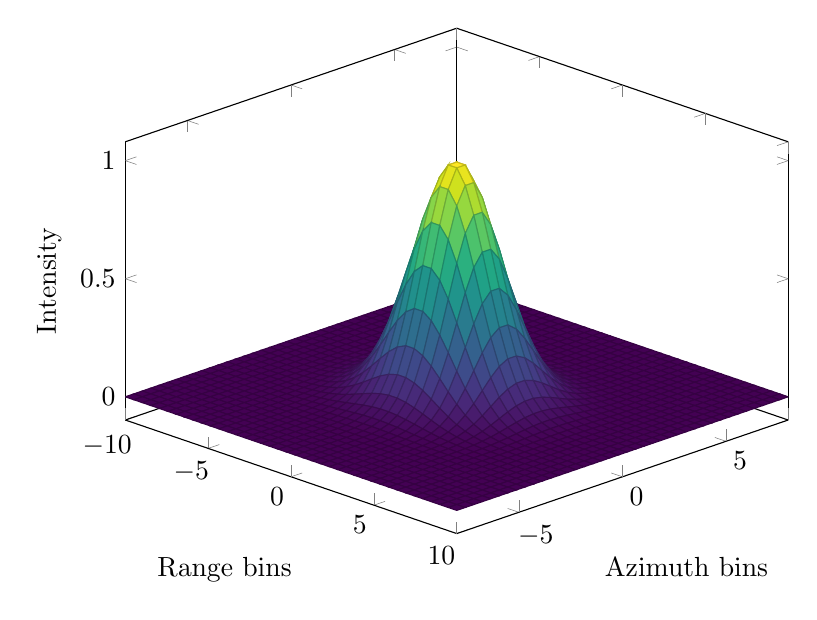
\begin{tikzpicture}
\begin{axis}[
    view={45}{30},
    width=10cm, height=8cm,
    xlabel={Range bins},
    ylabel={Azimuth bins},
    zlabel={Intensity},
    colormap/viridis,
]
    \addplot3[
        surf,
        domain=-10:10,
        domain y=-8:8,
        samples=40,
    ] {exp(-x^2/8 - y^2/4)};
\end{axis}
\end{tikzpicture}
\end{document}
